% Created by tikzDevice version 0.12.6 on 2024-02-19 10:08:16
% !TEX encoding = UTF-8 Unicode
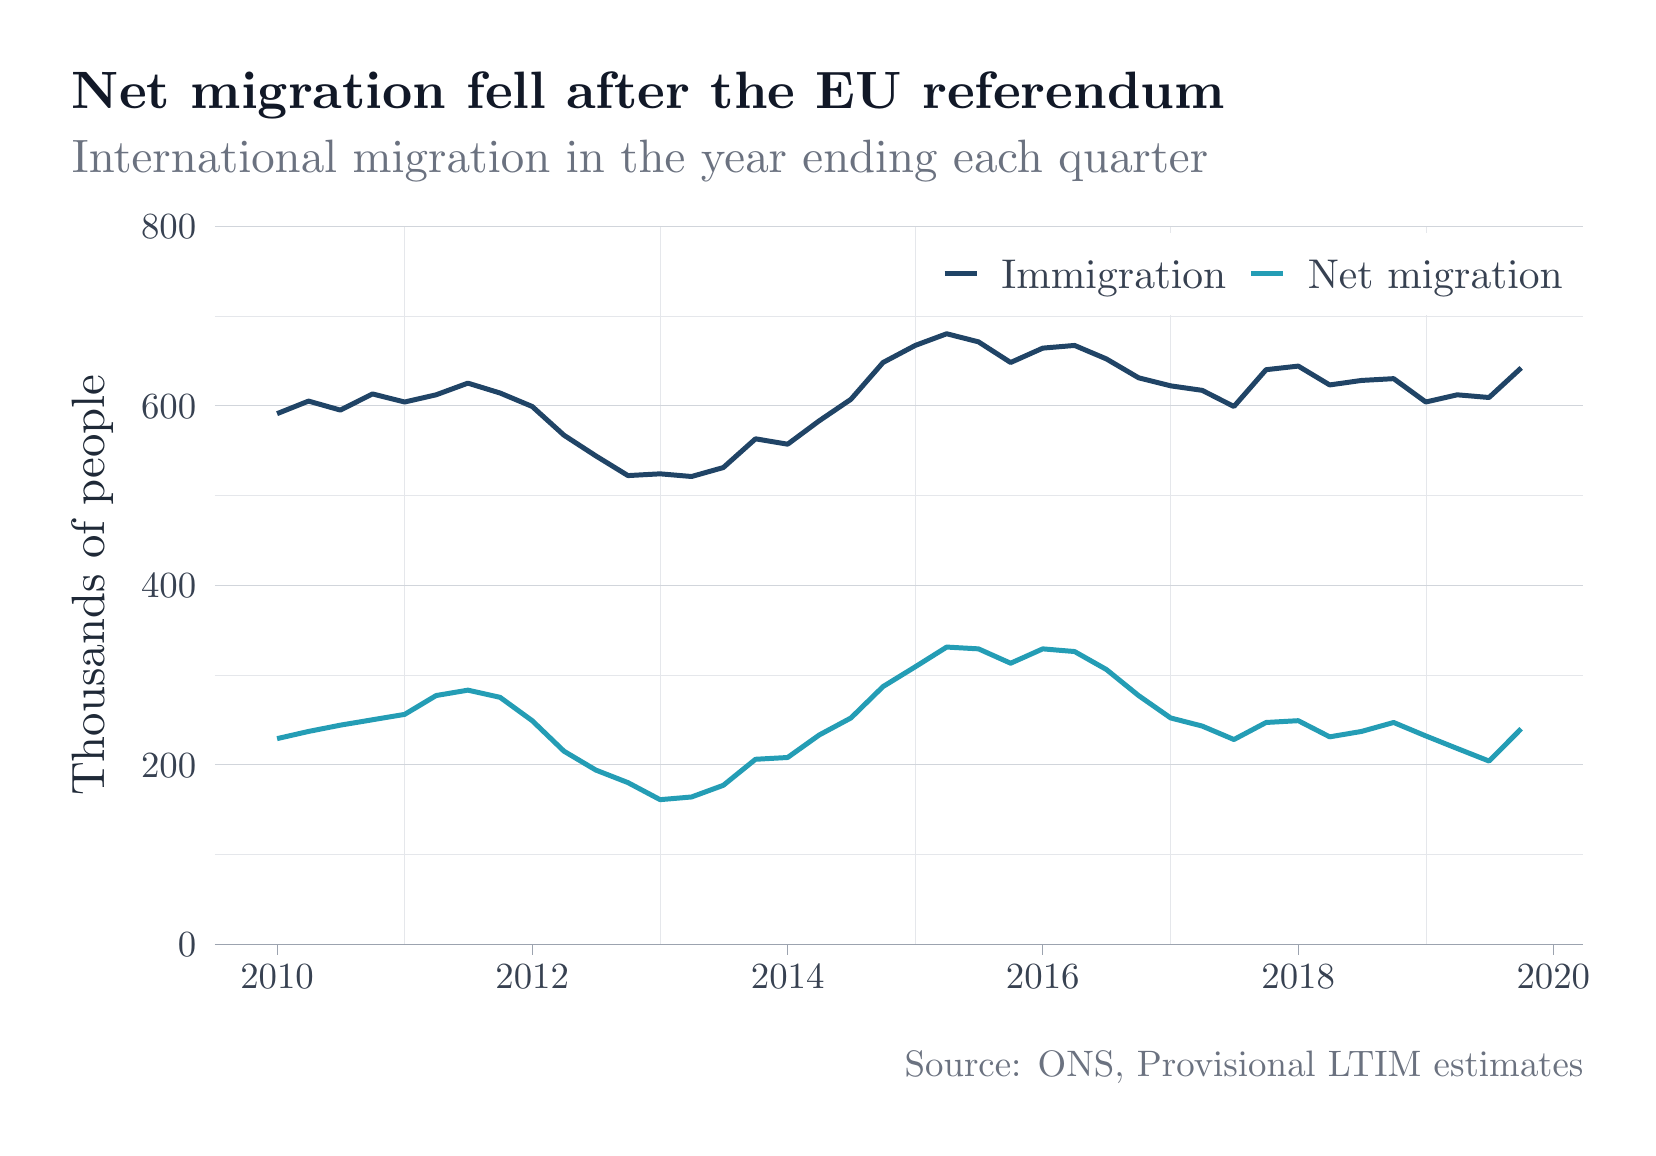
\begin{tikzpicture}[x=1pt,y=1pt]
\definecolor{fillColor}{RGB}{255,255,255}
\path[use as bounding box,fill=fillColor] (0,0) rectangle (578.16,397.48);
\begin{scope}
\path[clip] (  0.00,  0.00) rectangle (578.16,397.48);
\definecolor{drawColor}{RGB}{255,255,255}

\path[draw=drawColor,line width= 0.8pt,line join=round,line cap=round,fill=fillColor] ( -0.00,  0.00) rectangle (578.16,397.48);
\end{scope}
\begin{scope}
\path[clip] ( 67.65, 66.29) rectangle (562.16,325.79);
\definecolor{drawColor}{RGB}{255,255,255}
\definecolor{fillColor}{RGB}{255,255,255}

\path[draw=drawColor,line width= 0.8pt,line join=round,line cap=round,fill=fillColor] ( 67.65, 66.29) rectangle (562.16,325.79);
\definecolor{drawColor}{RGB}{229,231,235}

\path[draw=drawColor,line width= 0.2pt,line join=round] ( 67.65, 98.73) --
	(562.16, 98.73);

\path[draw=drawColor,line width= 0.2pt,line join=round] ( 67.65,163.60) --
	(562.16,163.60);

\path[draw=drawColor,line width= 0.2pt,line join=round] ( 67.65,228.48) --
	(562.16,228.48);

\path[draw=drawColor,line width= 0.2pt,line join=round] ( 67.65,293.35) --
	(562.16,293.35);

\path[draw=drawColor,line width= 0.2pt,line join=round] (136.22, 66.29) --
	(136.22,325.79);

\path[draw=drawColor,line width= 0.2pt,line join=round] (228.46, 66.29) --
	(228.46,325.79);

\path[draw=drawColor,line width= 0.2pt,line join=round] (320.71, 66.29) --
	(320.71,325.79);

\path[draw=drawColor,line width= 0.2pt,line join=round] (412.96, 66.29) --
	(412.96,325.79);

\path[draw=drawColor,line width= 0.2pt,line join=round] (505.21, 66.29) --
	(505.21,325.79);
\definecolor{drawColor}{RGB}{209,213,219}

\path[draw=drawColor,line width= 0.4pt,line join=round] ( 67.65, 66.29) --
	(562.16, 66.29);

\path[draw=drawColor,line width= 0.4pt,line join=round] ( 67.65,131.17) --
	(562.16,131.17);

\path[draw=drawColor,line width= 0.4pt,line join=round] ( 67.65,196.04) --
	(562.16,196.04);

\path[draw=drawColor,line width= 0.4pt,line join=round] ( 67.65,260.92) --
	(562.16,260.92);

\path[draw=drawColor,line width= 0.4pt,line join=round] ( 67.65,325.79) --
	(562.16,325.79);
\definecolor{drawColor}{RGB}{32,68,102}

\path[draw=drawColor,line width= 1.8pt,line join=round] ( 90.12,258.00) --
	(101.49,262.54) --
	(112.98,259.29) --
	(124.60,265.13) --
	(136.22,262.21) --
	(147.58,264.81) --
	(159.07,269.03) --
	(170.69,265.46) --
	(182.31,260.59) --
	(193.80,250.21) --
	(205.29,242.75) --
	(216.91,235.62) --
	(228.53,236.26) --
	(239.89,235.29) --
	(251.38,238.53) --
	(263.00,248.91) --
	(274.62,246.97) --
	(285.99,255.40) --
	(297.48,263.19) --
	(309.09,276.49) --
	(320.71,282.65) --
	(332.08,286.87) --
	(343.57,283.95) --
	(355.19,276.49) --
	(366.80,281.68) --
	(378.30,282.65) --
	(389.79,277.78) --
	(401.41,270.97) --
	(413.02,268.05) --
	(424.39,266.43) --
	(435.88,260.59) --
	(447.50,273.89) --
	(459.12,275.19) --
	(470.48,268.38) --
	(481.97,270.00) --
	(493.59,270.65) --
	(505.21,262.21) --
	(516.57,264.81) --
	(528.06,263.84) --
	(539.68,274.54);
\definecolor{drawColor}{RGB}{36,157,181}

\path[draw=drawColor,line width= 1.8pt,line join=round] ( 90.12,140.57) --
	(101.49,143.17) --
	(112.98,145.44) --
	(124.60,147.39) --
	(136.22,149.33) --
	(147.58,156.14) --
	(159.07,158.09) --
	(170.69,155.50) --
	(182.31,147.06) --
	(193.80,136.03) --
	(205.29,129.22) --
	(216.91,124.68) --
	(228.53,118.52) --
	(239.89,119.49) --
	(251.38,123.71) --
	(263.00,133.11) --
	(274.62,133.76) --
	(285.99,141.87) --
	(297.48,148.04) --
	(309.09,159.39) --
	(320.71,166.52) --
	(332.08,173.66) --
	(343.57,173.01) --
	(355.19,167.82) --
	(366.80,173.01) --
	(378.30,172.04) --
	(389.79,165.55) --
	(401.41,156.14) --
	(413.02,148.04) --
	(424.39,145.12) --
	(435.88,140.25) --
	(447.50,146.41) --
	(459.12,147.06) --
	(470.48,141.22) --
	(481.97,143.17) --
	(493.59,146.41) --
	(505.21,141.55) --
	(516.57,137.01) --
	(528.06,132.47) --
	(539.68,144.14);

\path[] ( 67.65, 66.29) rectangle (562.16,325.79);
\end{scope}
\begin{scope}
\path[clip] (  0.00,  0.00) rectangle (578.16,397.48);
\definecolor{drawColor}{RGB}{55,65,81}

\node[text=drawColor,anchor=base east,inner sep=0pt, outer sep=0pt, scale=  1.33] at ( 60.90, 61.70) {0};

\node[text=drawColor,anchor=base east,inner sep=0pt, outer sep=0pt, scale=  1.33] at ( 60.90,126.58) {200};

\node[text=drawColor,anchor=base east,inner sep=0pt, outer sep=0pt, scale=  1.33] at ( 60.90,191.45) {400};

\node[text=drawColor,anchor=base east,inner sep=0pt, outer sep=0pt, scale=  1.33] at ( 60.90,256.33) {600};

\node[text=drawColor,anchor=base east,inner sep=0pt, outer sep=0pt, scale=  1.33] at ( 60.90,321.20) {800};
\end{scope}
\begin{scope}
\path[clip] (  0.00,  0.00) rectangle (578.16,397.48);
\definecolor{drawColor}{RGB}{156,163,175}

\path[draw=drawColor,line width= 0.3pt,line join=round] ( 67.65, 66.29) --
	(562.16, 66.29);
\end{scope}
\begin{scope}
\path[clip] (  0.00,  0.00) rectangle (578.16,397.48);
\definecolor{drawColor}{RGB}{156,163,175}

\path[draw=drawColor,line width= 0.3pt,line join=round] ( 90.12, 62.54) --
	( 90.12, 66.29);

\path[draw=drawColor,line width= 0.3pt,line join=round] (182.31, 62.54) --
	(182.31, 66.29);

\path[draw=drawColor,line width= 0.3pt,line join=round] (274.62, 62.54) --
	(274.62, 66.29);

\path[draw=drawColor,line width= 0.3pt,line join=round] (366.80, 62.54) --
	(366.80, 66.29);

\path[draw=drawColor,line width= 0.3pt,line join=round] (459.12, 62.54) --
	(459.12, 66.29);

\path[draw=drawColor,line width= 0.3pt,line join=round] (551.30, 62.54) --
	(551.30, 66.29);
\end{scope}
\begin{scope}
\path[clip] (  0.00,  0.00) rectangle (578.16,397.48);
\definecolor{drawColor}{RGB}{55,65,81}

\node[text=drawColor,anchor=base,inner sep=0pt, outer sep=0pt, scale=  1.33] at ( 90.12, 50.36) {2010};

\node[text=drawColor,anchor=base,inner sep=0pt, outer sep=0pt, scale=  1.33] at (182.31, 50.36) {2012};

\node[text=drawColor,anchor=base,inner sep=0pt, outer sep=0pt, scale=  1.33] at (274.62, 50.36) {2014};

\node[text=drawColor,anchor=base,inner sep=0pt, outer sep=0pt, scale=  1.33] at (366.80, 50.36) {2016};

\node[text=drawColor,anchor=base,inner sep=0pt, outer sep=0pt, scale=  1.33] at (459.12, 50.36) {2018};

\node[text=drawColor,anchor=base,inner sep=0pt, outer sep=0pt, scale=  1.33] at (551.30, 50.36) {2020};
\end{scope}
\begin{scope}
\path[clip] (  0.00,  0.00) rectangle (578.16,397.48);
\definecolor{drawColor}{RGB}{31,41,55}

\node[text=drawColor,rotate= 90.00,anchor=base,inner sep=0pt, outer sep=0pt, scale=  1.69] at ( 27.63,196.04) {Thousands of people};
\end{scope}
\begin{scope}
\path[clip] (  0.00,  0.00) rectangle (578.16,397.48);
\definecolor{fillColor}{RGB}{255,255,255}

\path[fill=fillColor] (322.38,293.74) rectangle (562.16,323.20);
\end{scope}
\begin{scope}
\path[clip] (  0.00,  0.00) rectangle (578.16,397.48);
\definecolor{drawColor}{RGB}{255,255,255}
\definecolor{fillColor}{RGB}{255,255,255}

\path[draw=drawColor,line width= 0.8pt,line join=round,line cap=round,fill=fillColor] (329.88,301.24) rectangle (344.33,315.70);
\end{scope}
\begin{scope}
\path[clip] (  0.00,  0.00) rectangle (578.16,397.48);
\definecolor{drawColor}{RGB}{32,68,102}

\path[draw=drawColor,line width= 1.8pt,line join=round] (331.32,308.47) -- (342.89,308.47);
\end{scope}
\begin{scope}
\path[clip] (  0.00,  0.00) rectangle (578.16,397.48);
\definecolor{drawColor}{RGB}{255,255,255}
\definecolor{fillColor}{RGB}{255,255,255}

\path[draw=drawColor,line width= 0.8pt,line join=round,line cap=round,fill=fillColor] (440.60,301.24) rectangle (455.06,315.70);
\end{scope}
\begin{scope}
\path[clip] (  0.00,  0.00) rectangle (578.16,397.48);
\definecolor{drawColor}{RGB}{36,157,181}

\path[draw=drawColor,line width= 1.8pt,line join=round] (442.05,308.47) -- (453.61,308.47);
\end{scope}
\begin{scope}
\path[clip] (  0.00,  0.00) rectangle (578.16,397.48);
\definecolor{drawColor}{RGB}{55,65,81}

\node[text=drawColor,anchor=base west,inner sep=0pt, outer sep=0pt, scale=  1.50] at (351.83,303.30) {Immigration};
\end{scope}
\begin{scope}
\path[clip] (  0.00,  0.00) rectangle (578.16,397.48);
\definecolor{drawColor}{RGB}{55,65,81}

\node[text=drawColor,anchor=base west,inner sep=0pt, outer sep=0pt, scale=  1.50] at (462.56,303.30) {Net migration};
\end{scope}
\begin{scope}
\path[clip] (  0.00,  0.00) rectangle (578.16,397.48);
\definecolor{drawColor}{RGB}{107,114,128}

\node[text=drawColor,anchor=base west,inner sep=0pt, outer sep=0pt, scale=  1.69] at ( 16.00,345.07) {International migration in the year ending each quarter};
\end{scope}
\begin{scope}
\path[clip] (  0.00,  0.00) rectangle (578.16,397.48);
\definecolor{drawColor}{RGB}{17,24,39}

\node[text=drawColor,anchor=base west,inner sep=0pt, outer sep=0pt, scale=  1.90] at ( 16.00,368.39) {\bfseries Net migration fell after the EU referendum};
\end{scope}
\begin{scope}
\path[clip] (  0.00,  0.00) rectangle (578.16,397.48);
\definecolor{drawColor}{RGB}{107,114,128}

\node[text=drawColor,anchor=base east,inner sep=0pt, outer sep=0pt, scale=  1.33] at (562.16, 18.59) {Source: ONS, Provisional LTIM estimates};
\end{scope}
\end{tikzpicture}
